\documentclass[11pt]{article}
\usepackage{url,amsmath,setspace,amssymb,fullpage,color,varwidth,mdframed,mathtools}
\usepackage{enumitem}
\usepackage[n,advantage,operators,sets,adversary,landau,probability,notions,logic,ff,mm,primitives,events,complexity,asymptotics,keys]{cryptocode}
\usepackage{xcolor}
\usepackage{tikz}
\usetikzlibrary{shapes.geometric}


\newcommand{\heading}[5]{
   \renewcommand{\thepage}{#1-\arabic{page}}
   \noindent
   \begin{center}
   \framebox[\textwidth]{
     \begin{minipage}{0.9\textwidth} \onehalfspacing
       {\bf CS 601.442/642 -- Modern Cryptography} \hfill #2

       {\centering \Large #5

       }\medskip

       {\it #3 \hfill #4}
     \end{minipage}
   }
   \end{center}
}

\newcommand{\scribe}[4]{\heading{#1}{#2}{}{ #4}{ #3}}

%\setlength{\parindent}{0in}

\newcommand{\proof}{{\bf Proof. }} %% To begin a proof write \proof
\newcommand{\qed}{\mbox{}\hspace*{\fill}\nolinebreak\mbox{$\rule{0.6em}{0.6em}$}} %%to end your proof write $\qed$.
\newcommand{\ma}{{\mathcal A}}
\newtheorem{lemma}{Lemma}
\newtheorem{theorem}[lemma]{Theorem}
\newtheorem{definition}{Definition}
\newtheorem{proposition}{Proposition}
\newtheorem{remark}{Remark}
\newtheorem{assumption}{Assumption}
\bibliographystyle{plain}
\renewcommand{\sample}{\xleftarrow{\$}}
\newcommand{\Gen}{\mathsf{Gen}}
\newcommand{\Enc}{\mathsf{Enc}}
\newcommand{\Dec}{\mathsf{Dec}}
%\newcommand{\sk}{\mathsf{sk}}
%\newcommand{\pk}{\mathsf{pk}}
\newcommand{\Sign}{\mathsf{Sign}}
\newcommand{\Tag}{\mathsf{Tag}}
\newcommand{\Verify}{\mathsf{Verify}}
%\newcommand{\bin}{\{0,1\}}


\begin{document}
\scribe{1}{Instructor:
Abhishek Jain}{Homework 6}{Deadline: December 7; 2022, 1:30 PM EST}

\begin{enumerate}

\item \textbf{(15 points)} Let $\mathcal{E}=(\mathcal{E}.\mathsf{Gen},\mathcal{E}.\mathsf{Enc},\mathcal{E}.\mathsf{Dec})$ be an $\textbf{IND-CPA}$ secure secret key encryption scheme and $\mathcal{M}=(\mathcal{M}.\mathsf{Gen},\mathcal{M}.\mathsf{Tag},\mathcal{M}.\mathsf{Ver})$ be a \textbf{UF-CMA} secure MAC scheme. Consider the following encryption scheme $(\mathsf{KeyGen},\mathsf{Encrypt},\mathsf{Decrypt})$:
\begin{itemize}
    \item $\mathsf{KeyGen(1^{\lambda})}$: Generate $k_{\mathcal{E}}\leftarrow\mathcal{E}.\mathsf{Gen(1^{\lambda})}$ and $k_{\mathcal{M}}\leftarrow\mathcal{M}.\mathsf{Gen(1^{\lambda})}$. Output $k=(k_{\mathcal{E}},k_{\mathcal{M}})$

 \item $\mathsf{Encrypt}(k,m)$: Parse $k=(k_{\mathcal{E}},k_{\mathcal{M}})$. Compute $c'\leftarrow\mathcal{E}.\mathsf{Enc}(k_{\mathcal{E}},m)$, $\sigma\leftarrow\mathcal{M}.\mathsf{Tag}(k_{\mathcal{M}},c')$. Output $c=(c',\sigma)$.
\item $\mathsf{Decrypt}(k,c)$: Parse $k=(k_{\mathcal{E}},k_{\mathcal{M}})$ and $c=(c',\sigma)$. If $\mathcal{M}.\mathsf{Ver}(k_{\mathcal{M}},c',\sigma) \neq1$, output $\perp$. Else, output $m\leftarrow\mathcal{E}.\mathsf{Dec}(k_{\mathcal{E}},c')$.

\end{itemize}
Prove that this scheme is \textbf{IND-CCA2} secure.

\item \textbf{(10 points)} Let $(\mathsf{KeyGen},\mathsf{Encrypt},\mathsf{Decrypt})$ be an \textbf{IND-CCA2} secure public-key bit-encryption scheme. Consider the following encryption scheme $(\mathsf{KeyGen}',\mathsf{Encrypt}',\mathsf{Decrypt}')$ for $n$-bit messages. 

\begin{itemize}
    \item 
    $\mathsf{KeyGen'(1^{\lambda})}$: 
    For $i \in \{1,...,n\}$, generate $(\sk_i, \pk_i) \leftarrow \mathsf{KeyGen(1^\lambda)}$. Output $\pk = (\pk_1,...,\pk_n)$ and $\sk = (\sk_1,...,\sk_n)$

    \item
    $\mathsf{Encrypt}'(\pk,m)$: 
    Parse $\pk=(\pk_1,...,\pk_n)$ and parse $m=m_1\|...\|m_n$. For $i \in \{1,...,n\}$, compute $c_i\leftarrow\mathsf{Enc}(\pk_i,m_i)$. Output $c=(c_1,...,c_n)$.
    
    \item 
    $\mathsf{Decrypt}'(\sk,c)$: Parse $\sk=(\sk_1,...,\sk_n)$ and parse $c=(c_1,...,c_n)$. For $i \in \{0,...,n\}$, compute $m_i=\mathsf{Dec}(\sk_i,c_i)$. Output $m=m_1\|...\|m_n$.
\end{itemize}
Show that this scheme is not \textbf{IND-CCA2} secure.

\item \textbf{(15 points)} Suppose that Alice and Bob hold correlated inputs of the following form: Alice has $(r_0,r_1)$, where each $r_i \xleftarrow{\$} \bin$ and Bob has $(c,r_c)$, where $c \xleftarrow{\$} \bin$. 

Further suppose that at a later point, Alice and Bob wish to securely compute 1-out-of-2 OT with inputs $(x_0,x_1)$ and $b$ respectively. Show how Alice and Bob can use their correlated inputs for performing this task without using any cryptographic assumptions. That is, design a protocol for 1-out-of-2 OT that achieves {\em unconditional} security against semi-honest adversaries. Argue correctness and security of your protocol. (You don't need to give a full formal proof.) 

\iffalse
Consider the following two functionalities:
\begin{itemize}
	\item Special OT: This is a randomized, input-less functionality (i.e., the parties do not have any inputs) for two parties. Alice's output is $r_0,r_1$, where each $r_i \xleftarrow{\$} \bin$. Bob's output is $(c,r_c)$ where $c \xleftarrow{\$} \bin$.
	\item 1-out-of-2 OT: This is a two-party functionality where Alice's input consists of two bits $x_0, x_1$ and Bob's input is bit $b$. Bob's output is $x_b$ and Alice has no output.
\end{itemize}
Suppose Alice and Bob have a single sample of special OT. That is, Alice has $(r_0,r_1)$ and Bob has $(c,r_c)$. Now, Alice and Bob wish to securely compute 1-out-of-2 OT with inputs $(x_0,x_1)$ and $b$ respectively.

Design a two-party protocol for this task with security against semi-honest adversaries {\em without using any other assumptions.} Argue correctness and security of your protocol. You don't need to give a formal proof, just informal arguments will suffice. 
\fi
({\bf Hint:} Recall that one-time pads do not require any cryptographic assumptions.)

\item \textbf{(10 points)} Let Alice and Bob be two parties with inputs $a\in\mathbb{Z}_q$ and $b\in\mathbb{Z}_q$, respectively. They wish to check if their inputs are equal, i.e., whether $a=b$. They want to do this while making sure that they do not learn any other information about the other party's input. In other words, if $a\neq b$, then Alice should not learn $b$ and Bob should not learn $a$. 

Let $\mathbb{G}$ be a cyclic group of prime order $q$ with generator $g$. They run the following protocol:
\begin{itemize}
    \item Alice samples a random value $r\sample\mathbb{Z}_q$. It then computes $X=g^r$ and $Y=g^{ar}$. It sends $(X, Y)$ to Bob.
    \item Bob computes $X^b$. It outputs 1 if $X^b=Y$, and 0 otherwise. 
\end{itemize}
\textbf{Explain why this protocol is not secure against semi-honest Bob.}

\item \textbf{(15 points)} Let Alice and Bob have inputs $a$ and $b$, respectively. They want to securely send $(a+b)$ to a third-party Carol. Devise a protocol where Alice and Bob are only allowed to send \textbf{at most one message to each other} and \textbf{at most one message each to Carol}. Your protocol should satisfy all of the following security properties:
\begin{itemize}
    \item \textit{Security against Semi-honest Alice:} Alice should not learn $b$.
    \item \textit{Security against Semi-honest Bob:} Bob should not learn $a$.
    \item \textit{Security against Semi-honest Carol:} Carol should not learn $a$ and $b$.
\end{itemize}
{\bf Argue that your protocol indeed satisfies all three security conditions, and gives the correct output to Carol.} (You don't need to give a formal proof).

\item \textbf{(15 points)} Let $C$ be a Boolean circuit as shown in the following figure.  
	\begin{center}
		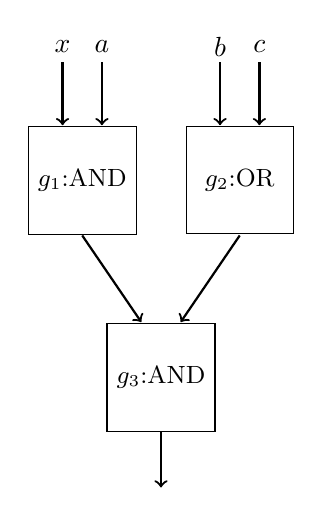
\begin{tikzpicture}[square/.style={regular polygon,regular polygon sides=4}]
        \node at (0,0) [square,draw] (v500) {\small{\textcolor{white}{AND}}};
        \node at (-0.25,1.7) {$x$};
        \draw[thick,->] (-0.25,1.5) -- (-0.25,0.7) ;
        \node at (0.25,1.7) {$a$};
        \draw[thick,->] (0.25,1.5) -- (0.25,0.7) ;
	    
	    \node at (2,0) [square,draw] (v900) {\small{\textcolor{white}{TOR}}};
        \node at (1.75,1.7) {$b$};
        \draw[thick,->] (1.75,1.5) -- (1.75,0.7) ;
        \node at (2.25,1.7) {$c$};
        \draw[thick,->] (2.25,1.5) -- (2.25,0.7) ;
        
        \node at (1,-2.5) [square,draw] (v500) {\small{\textcolor{white}{AND}}};
        \draw[thick,->] (0,-0.7) -- (0.75,-1.8) ;
        \draw[thick,->] (2,-0.7) -- (1.25,-1.8) ;
        \draw[thick,->] (1,-3.2) -- (1,-3.9) ;
        \node at (0,0) {\small $g_1$:AND};
        \node at (2,0) {\small $g_2$:OR};
        \node at (1,-2.5) {\small $g_3$:AND};
		\end{tikzpicture}
	\end{center}
	Let $(\mathsf{Garble},\mathsf{Eval})$ be the garbling scheme discussed in class. Recall that the $\mathsf{Garble}()$ function, when given this Boolean circuit $C$ as input, outputs the following:
$$
(\hat{G}=\{\hat{g_1},\hat{g_2},\hat{g_3}\}, \hat{\mathsf{In}}=\{K_0^1,K_1^1,K^2_0,K^2_1,K^3_0,K^3_1,K^4_0,K^4_1\})\gets\mathsf{Garble}(C),
$$
where $\hat{G}$ is the set of 3 garbled gates and 
$\hat{\mathsf{In}}$ is the set of wire keys for the 4 input wires in this circuit. In this question, we will see that the privacy of inputs in a garbled circuit does not hold if the adversary has both the keys for a wire.


Consider an adversary who knows the description of $C$, garbled gates $\hat{G}$ and input wire keys $\{K_0^1,K_1^1,K^2_a,K^3_b,K^4_c\}$. Note that the adversary gets both the input wire keys for the first input wire, and only one key for each of the remaining 3 input wires. Also note that the values $a,b,c$ are not known to the adversary.

\textbf{Show how this adversary can use this information to learn at least one out of $a$, $b$ or $c$.}

(\textbf{Hint: Use the truth table of the gates to derive information.})


\end{enumerate}
\end{document}
